\section{Function points}
The Function Point estimation approach is based on the amount of functionalities in a software and their complexity.
We will now provide a detailed description on the function points related to our application.

There are five estimators to take in account:
\begin{itemize}
	\item Internal logic files
	\item External interface files
	\item External inputs
	\item External outputs
	\item External inquiries
\end{itemize}

This table defines the weights values that we've to use to perform the FP value.
\begin{figure}[h]
	\centering
	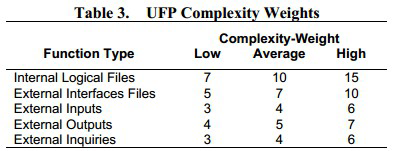
\includegraphics{tab1.png}
	\caption{Weights for all the different estimators}
\end{figure}

We will now proceed to identify all the elements and assign a value to them

\subsection{Internal Logic files}
An internal logic files is simply a data structure used in the application.
The ILFs of our system are the following:
\begin{itemize}
	\item User
	\item Passenger
	\item TaxiDriver
	\item Request
	\item Ride
\end{itemize}
User, passenger and taxi drivers can be assumed to be simple data structure. Request and ride are a little more complex so we'll treat them as average complexity.

\subsection{External interface files}
External Interface Files are a homogeneous set of data used by the application but generated by other applications.

The only EIF of our system is the interface of a map service we use for navigation. It can be considered as average complexity.

\subsection{External inputs}
External Inputs are operations to elaborate data coming from the external environment.
The EIs of our system are:
\begin{itemize}
	\item Registration
	\item Login
	\item Simple request
	\item Taxi reservation
	\item Driver availability
\end{itemize}
Login, request, reservation and driver availability are inputs with low complexity. Registration is more complex (average complexity)since it involves a bigger amount of data and components.

\subsection{External outputs}
External Output is an elementary operation that generates data for the external environment.
The EOs of our system are:
\begin{itemize}
	\item Notifications to users
	\item Notifications to taxi drivers
\end{itemize}
Both of this outputs can be considered of low complexity.

\subsection{External Inquiry}
External Inquiry is as an operation that involves input and output, without elaboration of data.
The EQs of the system are:
\begin{itemize}
	\item Taxi driver ride request
	\item Ride sharing
\end{itemize}
Ride request to taxi driver is simple (low complexity). On the other hand, ride sharing requires a lot of operations since it can be considered of high complexity.

\subsection{Summary}
\begin{description}
	\item[Internal logic files score:] 3 low complexity + 2 average complexity: $ 3*7 + 2*10 = 41$
	\item[External onterface files score:] 1 medium complexity: 7
	\item[External inputs score:] 4 low complexity + 1 average complexity: $4*3 + 1*4 = 16 $
	\item[External outputs score:] 2 low complexity: 4
	\item[External inquiries:] 1 low complexity + 1 high complexity: $1*3 + 1*6 = 9$ 
\end{description}
The total is of $41+7+16+4+9=77$

\subsection{Source lines of code}
The conversion multiplicator from function points to SLOC is 53 for the Java language: hence we have $77*53=4081$ lines of code.
